%\begin{savequote}[75mm]
%Nulla facilisi. In vel sem. Morbi id urna in diam dignissim feugiat. Proin molestie tortor eu velit. Aliquam erat volutpat. Nullam ultrices, diam tempus vulputate egestas, eros pede varius leo.
%\qauthor{Quoteauthor Lastname}
%\end{savequote}

\chapter{Metodología de Desarrollo para el Sistema}

\newthought{Desarrollo Guiado por Comportamiento} - BDD\footnote{BDD, por sus
siglas en inglés, Behaviour-Driven Development}, es la metodología que se eligió
para el desarrollo del Sistema.

Es una técnica de desarrollo ágil de software que fomenta la colaboración
entre desarrolladores, testers y clientes. Fue nombrado originalmente en el año
2003 por Dan North\footnote{Dan North, \url{http://dannorth.net/} consultado en
fecha 10/06/2014} en respuesta al Desarrollo Guiado por Pruebas - TDD\footnote{TDD,
por sus siglas en inglés, Test-Driven Development}. Podemos considerarlo una evolución
o un mejor entendimiento y una forma mejor de explicar los procesos TDD. Se observo
que los {\it desarrolladores} estaban teniendo momentos difíciles en relación
con TDD que es más una herramienta para diseño que para hacer pruebas.

%en el que el énfasis se pone más en las especificaciones
%finales del software antes que en sus detalles técnicos.

\section{Test-Driven Development - Donde todo empezó}
TDD es una practica de desarrollo que involucra escribir primero los {\it ``Test''}
antes que el código a ser {\it testeado} o probado. Se empieza escribiendo test
muy pequeños para el código que aun no existe, luego de esto si corremos los test
notaremos que los test fallan naturalmente, ahora hay que escribir el código
necesario para que el test pase.

Una vez que pase los tests, observe el diseño resultante, y refactorizar cualquier
duplicación o código innecesario que se encuentre. Es natural que en este momento
el diseño es demasiado simple para manejar todas las responsabilidades que tendrá.

En lugar de añadir mas código, documente la siguiente responsabilidad en el
formulario de los siguientes tests. Ejecútelo, y vea los fallos, escriba el código
necesario para que pase el test, revise el diseño, remueva el código innecesario
o duplicado. Ahora añada el siguiente test, vea los fallos, consiga que pase los
tests, refactorizar, fallo, paso, refactorizar, fallo, paso, refactorizar,
\ldots etc.

\begin{figure}[h]
  \begin{center}
  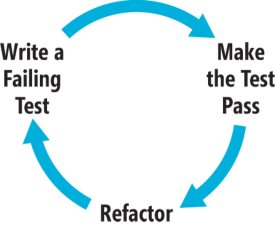
\includegraphics[width=0.4\textwidth]{figures/chapter2/tdd_cycle.jpg}
  \caption[TDD]{Ciclo del Desarrollo Guiado por Pruebas.}
\end{center}
\end{figure}
En muchos {\it Sistemas de Tests}, cuando un test falla, nosotros vemos los
resultados pintados en {\it rojo}. Después cuando esto pasa, los resultados
son pintados en {\it verde}. Debido a esto, a menudo nos referimos a este ciclo
como {\it rojo/verde/refactorizar}.

\begin{figure}[h]
  \centering
  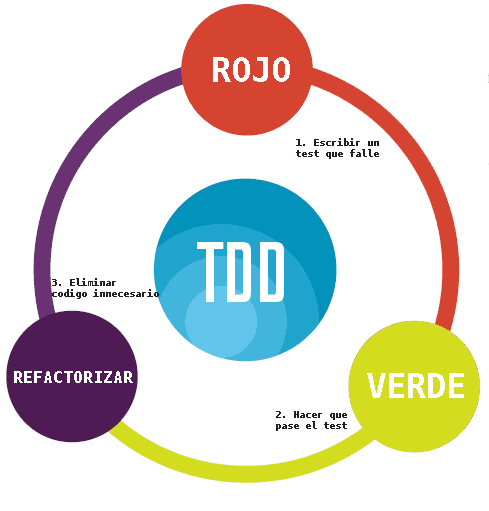
\includegraphics[width=0.6\textwidth]{figures/chapter2/tdd.png}
  \caption[TDD: red, green, refactor]{Desarrollo Guiado por Pruebas es rojo, verde, refactor.}
\end{figure}

\subsection{Diseño emergente}

Como el código base incrementa en tamaño, encontraron que se da mucha atención
en el paso de refactorización. El diseño esta en constante evolución y bajo
revisión constante, aunque no esta predeterminado. Esto es un {\it diseño
emergente} a un nivel granular y es uno de los subproductos mas significativos
de TDD.

Más que pensar en TDD como una práctica de pruebas, lo vemos como una técnica
utilizada para entregar código de alta calidad a los testers, los que son
responsables de las prácticas de pruebas formales.

Y aquí es donde los {\it Test} en TDD llega a tener problemas. Específicamente,
esta es la idea de {\it unit testing }\footnote{unit testing, son pruebas unitarias}
y esto a menudo conduce a nuevos TDDers para verificar y asegurarse de que un objeto
sea el objeto esperado, como ser un método {\it register()} almacene una colección
de {\it Registers} y sea específicamente un {\it Array}.

Este tipo de detalle en un test crea una dependencia del test en la estructura
interna del objeto que esta siendo probado. Esta dependencia significa, que si
hay otro requerimiento que nos hace cambiar el objeto de Array a Hash el test
fallará, a pesar de que el comportamiento no cambie. Esta fragilidad puede hacer
conjuntos de pruebas mucho mas caras de mantener, y esta es la razón por la que
muchos grupos de pruebas son ignorados o incluso descartados.

En resumen, si estos test internos que se hace a un objeto son contraproducente
a largo plazo, ?`en que debemos centrarnos al escribir estos test por primera vez?

\vspace{0.5cm}
\begin{mdframed}
{\it TDD es una práctica para entregar código de calidad con un buen diseño
  que una práctica para realizar {\bfseries pruebas}}
\end{mdframed}

\section{Behaviour-Driven Development: El siguiente paso}
El problema con los tests que se hacen a la estructura de los objetos es que
estamos probando si {\it es} un objeto en lugar de lo que {\it hace} el objeto. Lo que
{\it hace} un objeto es mucho más importante.

Lo mismo ocurre a nivel de aplicación. Los Stakeholders\footnote{Stakeholders,
los interesadas del sistema} no le dan importancia a que si los datos son
persistentes o no en una base de datos relacional compatible con ANSI. A ellos
les importa de que {\it ``estén en la base de datos''}, por lo general a ellos
les interesa de que este almacenado en {\it algún lugar} de donde ellos puedan
recuperarlo.

\subsection{Todo es Comportamiento}
BDD se enfoca completamente en el {\it comportamiento} en lugar de la estructura,
y lo hace en todos los niveles de desarrollo. Ya sea que estemos hablando de un
objeto que calcule la distancia entre dos ciudades, u otro objeto que delegue la
búsqueda de servicios, o una interfaz de usuario que se provee para hacer feedback
cuando ocurre una salida invalida, {\it todo es comportamiento}.

Una vez que reconocemos esto, cambiamos la forma en que pensamos acerca de la
expulsión de código. Empezamos a pensar mas en la interacción entre las personas
y el sistema, o entre objetos, de los que sabemos acerca de su estructura.

\subsection{Conseguir las Palabras Correctas}
Creemos que la mayoría de los problemas que enfrentan los equipos de desarrollo
de software son los problemas de comunicación. BDD tiene como objetivo ayudar a la
comunicación mediante la simplificación del lenguaje que usamos para describir los
escenarios en los que se utilizara el software: {\it Given} obtener datos de algún
contexto, {\it When} cuando ocurre algún evento, {\it Then} entonces espero algún
resultado.

{\it Given, When, Then}, la triada BDD, son simples palabras que utilizaremos ya
sea que estemos hablando del comportamiento de la aplicación o de un objeto. Estas
palabras son fáciles de entender por los analistas de negocios, testers, y
desarrolladores por igual. Estas palabras están incrustadas en el DSL\footnote{
Domain Specific Language, Lenguaje de dominio especifico} Gherkin.

\subsection{Gherkin}
Gherkin es un DSL legible para gente no técnica, que permite definir el
comportamiento del software sin detallar como está implementado, además de que
nos permite documentar las funcionalidades a la vez que escribimos casos de
prueba automáticos.

Otras ventajas que nos proporciona usar Gherkin:
\begin{itemize}
    \item Fácil de entender
    \item Fácil de leer
    \item Fácil de parsear
    \item Fácil de discutir
\end{itemize}

Gherkin es un lenguaje que usa el indentado para definir la estructura, de manera
que los saltos de linea dividen las diferentes declaraciones, la mayoría de las
lineas empiezan con palabras clave. El parser divide el texto en {\it Features,
Scenarios y Steps}, cuando pasas los casos de prueba, el parser busca un Step con
ese nombre. Los Steps son los análogos de los métodos en Java o las funciones en
Javascript.

La gramática de Gherkin consiste en pocas palabras claves que debe usarse cuando
escribimos un archivo {\it .feature}:

\begin{itemize}
    \item Feature
    \item Background
    \item Scenario
    \item Scenario outline
    \item Examples
    \item Given, When, Then, And, But (Para definir pasos)
    \item | (Para definir tablas)
    \item '''''' (Para definir una cadena de varias lineas)
    \item \# (Para usar comentarios)
\end{itemize}

Se puede escribir lo que uno quiere después de una palabra clave. Las palabras
claves {\it Given, When, Then, And} y {\it But} indican pasos en un escenario, que
usaremos para construir un DSL para un proyecto.

Cada {\it Feature} o {\it característica} se define en un archivo {\it .feature},
un característica normalmente consiste en una serie de {\it escenarios}, el texto
entre {\it Feature} y {\it Scenario} permite definir libremente el contexto ya
que este texto no será usado para ninguna funcionalidad en el código generado,
es meramente descriptivo.

\vspace{0.5cm}
\begin{mdframed}
\begin{alltt}
\emph{Feature:} [nombre de la característica en general a probar]
  \emph{As} [un actor/rol]
  \emph{In order to} [algún beneficio]
  \emph{I want} [una característica]

  \emph{Scenario:} \ldots
\end{alltt}
\end{mdframed}
\vspace{0.5cm}

Nos ayuda a entender {\it como} que tipo de usuario es el que va ha usar esta
característica o funcionalidad, {\it para} que nos sirve esta funcionalidad y que
{\it quiero} obtener.

\subsection{Scenario - Esquema del escenario}
Los escenarios son ejemplos concretos de como queremos que se comporte el software.
Esta manera de hacerlo es mas explicita que algunas formas tradicionales para
describir requerimientos y nos ayudan a plantear y responder preguntas que de lo
contrario no podríamos hacerlas. Los escenarios nos permiten responder a preguntas,
describiendo exactamente lo que debe suceder y en que circunstancias debe hacerse.
\newpage
\vspace{0.5cm}
\begin{mdframed}
\begin{alltt}
\emph{Feature:} [nombre de la característica en general a probar]
  \emph{As} [un actor/rol]
  \emph{In order to} [algún beneficio]
  \emph{I want} [una característica]

  \emph{Scenario:} [un ejemplo concreto de lo que se quiere probar]
\end{alltt}
\end{mdframed}
\vspace{0.5cm}

Cuando se empieza a escribir una nueva {\it característica} o {\it feature}, por
lo general es más fácil comenzar con un escenario que describe el ``camino feliz''
y más común. Una vez que haya terminado con eso, se puede agregar más escenarios
que describan diferentes casos, por ejemplo:

\vspace{0.5cm}
\begin{mdframed}
\begin{alltt}
\emph{Feature:} [nombre de la característica en general a probar]
  \emph{As} [un actor/rol]
  \emph{In order to} [algún beneficio]
  \emph{I want} [una característica]

  \emph{Scenario:} [un ejemplo concreto de lo que se quiere probar]

  \emph{Scenario:} [\ldots]

  \emph{Scenario:} [\ldots]

  \ldots
\end{alltt}
\end{mdframed}
\vspace{0.5cm}

Ahora, para que cada {\it Scenario} tenga un comportamiento correcto necesita
seguir varios pasos.

\subsection{Steps - Pasos}
Cada escenario usa un numero arbitrario de {\it pasos} o {\it steps} para describir
todo lo que pasa dentro de un escenario. Un paso es generalmente una simple linea
de texto que empieza con una de las palabras claves: {\it Given, When, Then, And}
y {\it But}
\newpage
\vspace{0.5cm}
\begin{mdframed}
\begin{alltt}
\emph{Feature:} [nombre de la característica en general a probar]
  \emph{As} [un actor/rol]
  \emph{In order to} [algún beneficio]
  \emph{I want} [una característica]

  \emph{Scenario:} [un ejemplo concreto de lo que se quiere probar]
    \emph{Given} [una condición previa]
    \emph{When} [una acción]
    \emph{Then} [un resultado esperado]

  \emph{Scenario:} [\ldots]
    \emph{Given} [\ldots]
    \emph{When} [\ldots]
    \emph{Then} [\ldots]

  \emph{Scenario:} [\ldots]

  \emph{Scenario:} [\ldots]
\end{alltt}
\end{mdframed}
\vspace{0.5cm}

\subsection{Internacionalización}
Las palabras reservadas de Gherkin fueron traducidas en varios idiomas como el
español, eso significa que nosotros podemos escribir los {\it Features} en nuestro
propio idioma o en el idioma del stakeholder. En los archivos {\it .feature} se
debe escribir la siguiente linea en la cabecera del archivo.
\begin{verbatim}
# language: es
Característica: [...]
\end{verbatim}

Para otros idiomas como el frances o portugues seria de la siguiente forma:

\begin{verbatim}
# language: fr
Fonctionnalité: [...]

# language: pt
Funcionalidade: [...]
\end{verbatim}
Gherkin usa por defecto el idioma ingles, asi que no es necesario poner la cabecera
si es que se va ha escribir en ingles.

Con la cabecera ya puesta en español, podemos escribir los features de la siguiente
manera:

\vspace{0.5cm}
\begin{mdframed}
\begin{alltt}
# language: es

\emph{Característica:} [nombre de la característica en general a probar]
  \emph{Como} [un actor/rol]
  \emph{Para} [algún beneficio]
  \emph{Quiero} [una característica]

  \emph{Esquema del escenario:} [un ejemplo concreto a probar]
    \emph{Dado} [una condición previa]
    \emph{Cuando} [una acción]
    \emph{Entonces} [un resultado esperado]

  \emph{Esquema del escenario:} [\ldots]
    \ldots
  \emph{Esquema del escenario:} [\ldots]
    \ldots

\end{alltt}
\end{mdframed}

\newpage
\section{El ciclo de BDD}
BDD se centra en la obtención de una comprensión clara del comportamiento del
software deseado a través de la discusión con las partes interesadas.

Es una forma de crear comportamientos o funcionalidades que se puedan probar y
sean automatizados que agreguen valor al momento de mostrar al cliente antes de
que exista el código fuente. Evitan errores que pudieran existir basados en las
funcionalidades o comportamientos del sistema y generan un conjunto de tests
basados en esas funcionalidades.

Según \citeauthor{BDDinAction} define de una forma
clara el funcionamiento básico de BDD:

\begin{figure}[h]
  \begin{center}
  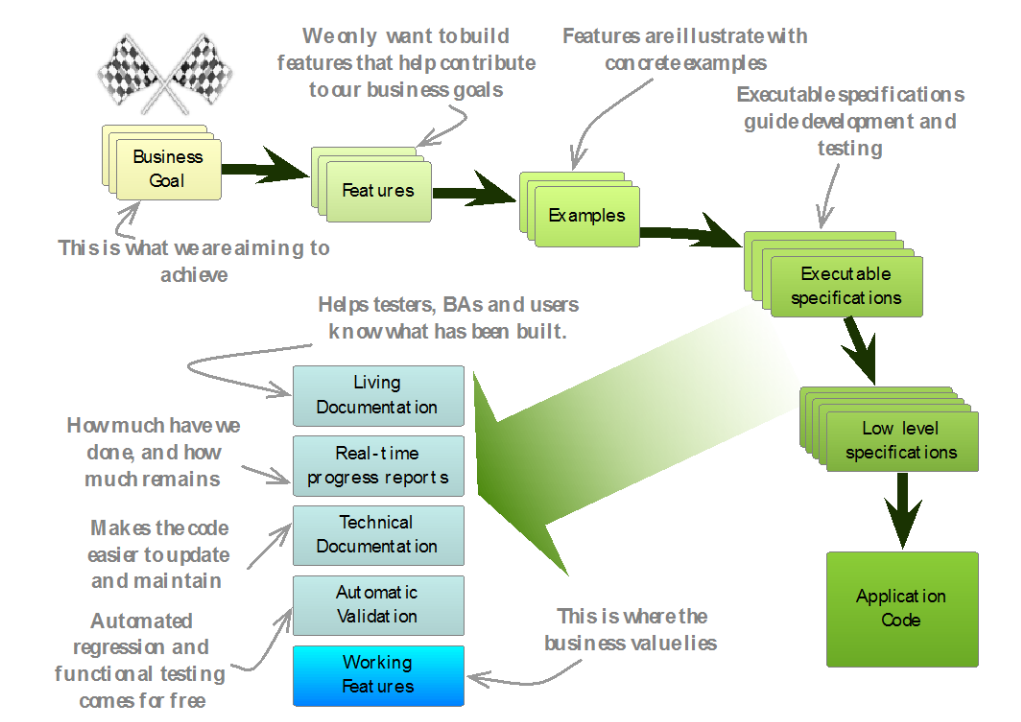
\includegraphics[width=1\textwidth]{figures/chapter3/bddinaction.png}
  \caption[BDD]{Funcionamiento Básico de BDD, Fuente: John Ferguson Smart - BDD in Action}
\end{center}
\end{figure}

\begin{mdframed}
  \centering
  Hacer que pase un test es {\it muy diferente} a una funcionalidad conseguida.
\end{mdframed}

\newpage
Con lo expuesto anteriormente llegamos a un ciclo ágil de desarrollo:

\begin{figure}[h]
  \begin{center}
  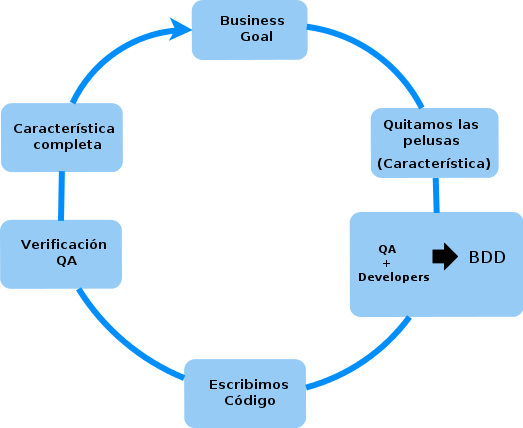
\includegraphics[width=0.7\textwidth]{figures/chapter2/bdd_cycle2.png}
  \caption[BDD]{El ciclo de vida ágil de BDD}
\end{center}
\end{figure}

Las historias o los {\it Business Goal} son los que dirigen nuestro desarrollo,
estas historias son parte de nuestro desarrollo, son las funcionalidades que
queremos conseguir.

Una vez que lo hemos implementado podemos comprobar de acuerdo con las
especificaciones que se han escrito al principio.

En el siguiente capítulo veremos a detalle el funcionamiento de BDD con escenarios
reales.

\section{Herramientas para BDD}
Gherkin tiene varias opciones que interpretan su código escritos en los archivos
{\it .feature} tales como: Cucumber, Lettuce, Freshen, Behave, etc.

Para este proyecto usamos Behave\footnote{Behave, desarrallado por \citeauthor{website:behave}}.

\subsection{Behave}
Behave es escribir BDD al estilo de Python, es decir behave utiliza los tests
escritos en un estilo de lenguaje natural como es Gherkin para obtener el código
inicial para hacer las pruebas que es código python y estas mismas son ejecutadas
para sus pruebas por behave.

En el siguiente capítulo se explicará con más detalle como se escriben las
funcionalidades y escenarios de prueba y como se los ejecuta con behave, tomando
en cuenta escenarios reales.

%\begin{mdframed}
%  BDD (Behavior-Driven Development): Forma de criar comportamentos testáveis e
%  automatizados que agreguem valor para o cliente antes da existência do código-fonte,
%  evitam defeitos baseados em comportamento e geram um conjunto de testes de
%  regressao baseados nesses comportamentos.
%\end{mdframed}

%% FIN DEL CAPITULO %%

\begin{comment}
Considere este requerimiento: {\it no debería
ser posible reservar una habitación si el hotel esta lleno}

Esto deja muchas preguntas abiertas. Si el hotel esta lleno, ¿es aun posible
tratar de reservar y obtener un error si lo intentamos? ¿esta deshabilitado la
opción de la reserva? o ¿esta oculto? ¿Que es lo que mostramos?

Los escenarios nos permiten responder a estas preguntas, describiendo exactamente
lo que debe suceder y en que circunstancias debe hacerse. Nuestro ejemplo quedaría
de la siguiente forma:

\vspace{0.5cm}
\begin{mdframed}
\begin{alltt}
# language: es

\emph{Característica:} Reservas de habitación para viajeros
  \emph{Como} propietario del hotel
  \emph{Para} reducir el hacinamiento
  \emph{Quiero} que los viajeros puedan disponer de habitaciones en la web

  \emph{Esquema del escenario:} Reserva exitosa
\end{alltt}
\end{mdframed}
\vspace{0.5cm}

Cada escenario se compone de pasos o {\it steps} que aparecen a continuación de
la palabra clave {\it Scenario} o {\it Esquema del escenario}. De esto hablaremos
en la siguiente sección.

Cuando se empieza a escribir una nueva {\it característica} o {\it feature}, por
lo general es más fácil comenzar con un escenario que describe el ``camino feliz''
y más común. Una vez que haya terminado con eso, se puede agregar más escenarios
que describan diferentes casos, por ejemplo:

\vspace{0.5cm}
\begin{mdframed}
\begin{alltt}
# language: es

\emph{Característica:} Reservas de habitación para viajeros
  \emph{Como} propietario del hotel
  \emph{Para} reducir el hacinamiento
  \emph{Quiero} que los viajeros puedan disponer de habitaciones en la web

  \emph{Esquema del escenario:} Reserva exitosa

  \emph{Esquema del escenario:} El hotel esta lleno

  \emph{Esquema del escenario:} El visitante se olvida introducir su e-mail
\end{alltt}
\end{mdframed}
\vspace{0.5cm}
\end{comment}

\begin{comment}
que entiende Cucumber\footnote{Cucumber, interpreta código
escrito en Gherkin en archivos {\it .feature}, fue la primer herramienta que se
hizo para BDD, las demas como behave, lettuce, freshen, se basaron en cucumber},

BDD se centra en la obtención de una comprensión clara del comportamiento del
software deseado a través de la discusión con las partes interesadas. Se extiende
de TDD escribiendo casos de prueba en un lenguaje natural que los no programadores
pueden leer. Los Desarrolladores que usan BDD usan su lengua materna en combinación
con un lenguaje específico y definido que sigue una sintaxis que es procesable y
automatizable para describir el propósito y beneficio de su código, el lenguaje en
el que se describe se llama Gherkin que es un DSL(Domain Specific Language).

Esto permite a los desarrolladores centrarse en por qué se debe crear el código, en lugar de los

detalles técnicos, y minimiza la traducción entre el lenguaje técnico en el que se escribe el
código y el lenguaje de dominio hablado por los usuarios, grupos de interés, gestión de proyectos,
etc.

Veamos un ejemplo: El titular de una cuenta quiere retirar dinero de un cajero automático cuando
el banco este cerrado.

\begin{alltt}
    \emph{Feature:} El cliente retira dinero del cajero

    \emph{As an} Cliente
    \emph{I want} retirar dinero del cajero autom\'atico
    \emph{So that} Quiero sacar dinero cuando el banco este cerrado

    \emph{Scenario}: La cuenta tiene el dinero suficiente
        \emph{Given} el saldo de la cuenta es de 100\$us
        \emph{And} la tarjeta es valida
        \emph{And} el cajero autom\'atico tiene el dinero suficiente
        \emph{When} el cliente inserta su tarjeta
        \emph{And} el cliente solicita 20\$us
        \emph{Then} el cajero autom\'atico debe dispensar 20\$us
        \emph{And} el saldo de la cuenta deber\'a ser de 80\$us
        \emph{And} la tarjeta debe ser devuelto

    \emph{Scenario}: \ldots
\end{alltt}

Utilizando la herramienta adecuada dependiendo el lenguaje de programaci\'on que uno este usando
se gener\'a el c\'odigo, en nuestro caso es Python y usaremos {\it behave}\footnote{Behave: \url{http://pythonhosted.org/behave/philosophy.html}}.

El c\'odigo que es generado son como especificaciones de lo que se quiere hacer, nos dice
que es lo que tenemos que programar para tener esa funcionalidad.

A diferencia de TDD que es una metodolgia m\'as de dise\~no y no de pruebas, BDD empieza haciendo las
funcionalidades que deben ser probadas, es una programaci\'on de afuera hacia adentro.

\vspace{1cm}

\begin{mdframed}
{\it BDD is a second-generation, outside–in, pull-based, multiple-stakeholder, multiple-scale,
 high-automation, agile methodology. It describes a cycle of interactions with well-defined outputs,
 resulting in the delivery of working, tested software that matters.}
\end{mdframed}

\vspace{1cm}

\begin{mdframed}
{\it BDD es una segunda generación, de afuera hacia adentro, con base extraíble, de múltiples
 partes interesadas, a escala múltiple, alta automatización, metodología ágil. En él se describe
 un ciclo de interacciones con productos bien definidos, lo que resulta en la entrega de trabajo,
 el software probado que importa.}
\end{mdframed}
\end{comment}


